%%%%%%%%%%%%%%%%%%%%%%%%%%%%%%%%%%%%%%%%%%%%%%%%%%%%%%%%%%%%%%%%%%%%%%%%%%%%%%%%%%%%%%%%%%%%%%%%%%%
%%%%%%%%%%%%%%%%%%%%%%%%%%%%%%%%%%%%%%%%%%%%%%%%%%%%%%%%%%%%%%%%%%%%%%%%%%%%%%%%%%%%%%%%%%%%%%%%%%%
%%%%%%%%%%%%%%%%%%%%%%%%%%%%%%%%%%%%%%%%%%%%%%%%%%%%%%%%%%%%%%%%%%%%%%%%%%%%%%%%%%%%%%%%%%%%%%%%%%%
%%%%%%%%%%%%%%%%%%%%%%%%%%%%%%%%%%%%%%%%%%%%%%%%%%%%%%%%%%%%%%%%%%%%%%%%%%%%%%%%%%%%%%%%%%%%%%%%%%%

\chapter{Metodología y resultados}
\label{ch:metodologia}

El presente trabajo surge de una colaboración con el Laboratorio de Sueño, Emoción y Cognición, dependiente del Instituto de Ciencias de la Salud de la UAEH y a cargo de la Dra. Alejandra Rosales Lagarde.
%
La colaboración incluye acceso a los registros obtenidos en un estudio por Vázquez-Tagle en 2016 \cite{VazquezTagle16}. 
%
Dicho estudio se centró en la epidemiología de los trastornos del sueño en adultos mayores dentro del estado de Hidalgo, y consideró registros de PSG para evaluar parámetros relacionados al sueño MOR.
%
El presente trabajo tiene como objetivo particular analizar con mayor detalle dichos registros.

En este capítulo se describe primeramente la metodología seguida para obtener los registros de PSG.
%
Posteriormente se describe la metodología usada para analizar los registros de PSG, usando las herramientas descritas en el capítulo \ref{capitulo:espectro_evo}.

Los registros de PSG fueron segmentados en ventanas de 30 segundos, referidas como \textbf{épocas}.
%
El análisis de los registros de PSG se llevó a cabo a tres niveles:
\begin{itemize}
\item Dentro de cada época.
\item Entre las diferentes épocas en un registro.
\item Entre los diferentes participantes.
\end{itemize}

El análisis a nivel de época contempla su clasificación según etapa de sueño (limitada a MOR y NMOR), y su clasificación como estacionarias (usando la prueba de PSR).
%
El uso de épocas como unidades de estudio se justifica por la gran heterogeneidad del sueño nocturno; paralelamente, destaca el supuesto fisiológico de que las etapas de sueño son \textit{comunes} entre los humanos.
%
En suma, los registros de PSG para un sólo individuo pueden interpretarse como una población de épocas.

El análisis a nivel de registro surge de considerar la heterogeneidad del sueño pero usando al registro entero como unidad de estudio.
%
El tomar las épocas junto con su estructura temporal reveló algunos patrones interesantes de actividad.

Para el análisis entre participantes (divididos en grupos), varias de las características descritas fueron \textit{colapsadas} para constituir características \textit{simples}. 
%
Debido a las características de la muestra (ver más adelante), los resultados obtenidos no pueden extrapolarse a la población en general.
%
Los resultados obtenidos, entonces, se presentan como \textit{indicios}.

%%%%%%%%%%%%%%%%%%%%%%%%%%%%%%%%%%%%%%%%%%%%%%%%%%%%%%%%%%%%%%%%%%%%%%%%%%%%%%%%%%%%%%%%%%%%%%%%%%%

\section{Características de los participantes}

Los participantes fueron elegidos usando un muestreo \textit{no probabilístico por conveniencia} bajo los siguientes criterios de inclusión:
\begin{itemize}
\item Edad entre 60 y 85 años
\item Diestros (mano derecha dominante)
\item Sin ansiedad, depresión ni síndromes focales
\item No usar medicamentos o sustancias para dormir
\item Firma de consentimiento informado
\item Voluntario para el registro de PSG
\end{itemize}

Un total de 16 adultos mayores cumplieron los criterios de inclusión. 
%
Con el fin de detectar el DCL en estos pacientes, éstos fueron sometidos a una batería de pruebas neuropsicológicas para determinar su estado cognoscitivo general (Neuropsi, MMSE), detectar cambios en su vida cotidiana (KATZ) y descartar cuadros depresivos (SAST, GDS); para más detalles ver capítulo anterior, sección \ref{seccion:pruebas}.
%
En la tabla \ref{tab_sujetos} se reportan los puntajes obtenidos por los participantes en dichas pruebas; estos datos deben ser interpretados según los \textit{puntajes de corte} de cada prueba, que se incluyen en el apéndice \ref{apendice_pruebas}.
%reportados en las tablas \refrange{anexo:sast_gds,anexo:mmse,anexo:neuropsi,anexo:katz}.
% \crefrange{anexo:sast_gds,anexo:mmse,anexo:neuropsi,anexo:katz}.
%
Se determinó que 11 de los voluntarios no padecen depresión o ansiedad, ni presentan afectaciones significativas en la vida diaria; el participante MGG presenta un cuadro depresivo, pero fue incluido en ausencia de afecciones cognitivas objetivas.
%
Debido a motivos técnicos, sólo 9 participantes fueron considerados para el presente trabajo; se reportan únicamente los datos relativos a esos participantes.

En base al diagnóstico de Posible Deterioro Cognitivo Leve, los 9 participantes fueron divididos en dos grupos: PDCL y CTRL. 
%
Es importante mencionar que, bajo las condiciones muestrales, el grupo CTRL no puede fungir satisfactoriamente como grupo control; una descripción más adecuada sería \textit{grupo sin PDCL}.

%Para esta clasificación se dio mayor atención al puntaje de Neuropsi, estandarizado según edad y 
%escolaridad (cuadro \ref{puntajes}). 
%
%Cabe mencionar que intencionalmente se dio menor importancia a los puntajes de la prueba MMSE en cuanto al diagnóstico del PDCL; ésto porque se ha reportado que, en la población mexicana, esa prueba tiene baja sensibilidad para el diagnóstico de DCL en general, y baja especificidad para individuos con escolaridad muy baja o muy alta \cite{Ostrosky00}.
%%
%Para fines del comentario anterior, se entiende por \textit{sensibilidad} a la probabilidad de obtener verdaderos positivos, y por \textit{especificidad} a la probabilidad de obtener verdaderos negativos.

\begin{table}
\caption{Datos generales de los participantes}
\centering
\bordes{1.1}
{\small
\begin{tabular}{llcrrrrrrr}
\toprule
 \phantom{mmm}&
 & {Sexo} & {Edad} & {Escol.} & {Neuropsi} & {MMSE} & {SAST} & {KATZ} & {GDS} \\
\midrule
\multicolumn{2}{l}{\textbf{Grupo CTRL}}\\
&MJH    & F    & 72\pz & 9\pz  & 113\pz & 30\pz & 18\pz & 0\pz & 0\pz  \\
&JAE    & F    & 78\pz & 5\pz  & 102\pz & 28\pz & 19\pz & 0\pz & 5\pz  \\
&MGG    & F    & 61\pz & 9\pz  & 114\pz & 28\pz & 29\pz & 1\pz & 14\pz \\
&EMT    & F    & 50\pz & 22\pz & 117\pz & 30\pz & 15\pz & 0\pz & 4\pz  \\
\rowcolor{gris}
&\multicolumn{1}{c}{$\widehat{\mu}$} & 
               & 65.3  & 11.3  & 111.5  & 29.0  & 20.3  & 0.3  & 5.8  \\
\rowcolor{gris}
&\multicolumn{1}{c}{$\widehat{\sigma}$} & 
               & 12.4  & 7.4   & 6.6    & 1.2   & 6.1   & 0.5  & 5.9  \\
\midrulec
%\hline
\multicolumn{2}{l}{\textbf{Grupo PDCL}}\\
& CLO   & F    & 68\pz &  5\pz &  81\pz & 28\pz & 22\pz & 1\pz &  6\pz \\
& RLO   & F    & 63\pz &  9\pz &  90\pz & 29\pz & 20\pz & 0\pz &  3\pz \\
& JGZ   & M    & 65\pz & 11\pz &  87\pz & 25\pz & 20\pz & 0\pz &  1\pz \\
& AEFP  & M    & 73\pz &  8\pz &  96\pz & 29\pz &   \pz & 0\pz &  2\pz \\
& PCM   & M    & 71\pz &  9\pz & 111\pz & 28\pz & 20\pz & 0\pz & 10\pz \\
\rowcolor{gris}
&\multicolumn{1}{c}{$\widehat{\mu}$} & 
              &  68.0  & 8.4   & 93.0   & 27.8  & 20.5  & 0.2  & 4.4  \\
\rowcolor{gris}
&\multicolumn{1}{c}{$\widehat{\sigma}$} & 
              & 4.1    & 2.2   & 11.4   & 1.6   & 1.0   & 0.4  & 3.6 \\
\bottomrulec
\end{tabular} 
}
\label{tab_sujetos}
\end{table}

%%%%%%%%%%%%%%%%%%%%%%%%%%%%%%%%%%%%%%%%%%%%%%%%%%%%%%%%%%%%%%%%%%%%%%%%%%%%%%%%%%%%%%%%%%%%%%%%%%%
%%%%%%%%%%%%%%%%%%%%%%%%%%%%%%%%%%%%%%%%%%%%%%%%%%%%%%%%%%%%%%%%%%%%%%%%%%%%%%%%%%%%%%%%%%%%%%%%%%%

\subsection{Registro del polisomnograma}

Para efectuar el registro de la PSG, los participantes acudieron a las instalaciones del Laboratorio de Sueño, Emoción y Cognición. 
%
Los participantes recibieron instrucciones de realizar una rutina normal de actividades durante la semana que precedió al estudio, y se les recomendó no ingerir bebidas alcohólicas o energizantes (como café o refresco) durante las 24 horas previas al experimento, y que no durmieran siesta ese día.
%
Bajo estas condiciones experimentales se garantiza que los registros son representativos del sueño nocturno de cada participante.

El registro per se fue efectuado usando un polisomnógrafo Medicid 5 (Neuronic Mexicana). El protocolo de la PSG incluye los siguientes electrodos\footnote{Para más detalles ver el capítulo anterior, particularmente la sección \ref{capitulo:psg}}:
\begin{itemize}
\item 19 electrodos de EEG colocadas según el Sistema Internacional 10--20.
\item 2 electrodos de EOG para movimientos oculares.
\item 2 electrodos de EMG para tono muscular en los músculos submentonianos.
\end{itemize}

Los electrodos para EEG fueron conectados en paralelo usando como referencia común los lóbulos de las orejas; se mantuvo por debajo de \SI{50}{\micro\ohm}.
%
Las señales fueron amplificadas analógicamente usando amplificadores de alta ganancia en cadena, 
y adicionalmente fueron \textit{pasado} filtros analógicos pasa bandas: 0.1--100 Hz 
para EEG, 3--20 Hz para EOG. 
%
Los registros fueron digitalizados con una frecuencia de muestreo de 512 puntos por segundos (Hz), y posteriormente almacenados en formato de texto bajo la codificación ASCII.

Como se mencionó anteriormente, los registros fueron segmentados en segmentos de 30 segundos, referidas como \textbf{épocas}; en lo posterior se usará la palabra `época' como un caso particular de ventana.
%
Cada una de las épocas fue clasificada como MOR o NMOR; la clasificación fue llevada a cabo por dos expertos de ICSA, y bajo los estándares de la AASM.

Por simplicidad técnica, los registros fueron truncados para poder considerar épocas completas; algunos datos al final de cada registro fueron omitidos, aunque representan una cantidad negligible de tiempo.
%
Cabe mencionar que cada época de 30 segundos, a una frecuencia de 512 Hz, representa un total de 15,360 puntos.

En la tabla \ref{tab:psg} se describe la duración de los registros, así como la cantidad de tiempo del registro clasificado como sueño MOR.
%
La cantidad de tiempo en vigilia registrado es negligible ($<5$ minutos por cada participante), de modo que ésta no es reportada; con una pérdida mínima de generalidad, se puede afirmar que los registros fuera del sueño MOR corresponden a sueño NMOR.

\begin{table}
\centering
\caption{Datos generales sobre los registros de PSG}
\bordes{1.2}
\begin{tabular}{llllcllr}
\toprule
    \phantom{mmm}&
    & \multicolumn{2}{l}{Total} & \phantom{l}   & \multicolumn{3}{l}{MOR*}\\
    \cmidrule{3-4}  \cmidrule{6-8}
    &          &Épocas  &  Tiempo   &&Épocas  &  Tiempo   &  \% \\
\midrule
\multicolumn{2}{l}{\textbf{Grupo CTL}}\\
&MJH &    1032   &      8:36:00  &&    127   &   1:03:30 &12.31 \\
&JAE &\ppu 904   &      7:32:00  &&    171   &   1:25:30 &18.92 \\
&MGG &    1024   &      8:32:00  &&    166   &   1:23:00 &16.21 \\
&EMT &\ppu 552   &      4:36:00  &&\ppu 47   &   0:23:00 & 8.51 \\
 
\rowcolor{gris}
&\multicolumn{1}{c}{$\widehat{\mu}$}  
     &\ppu 878.0 &      7:19:00 &&    128.0 &   1:03:53&13.99 \\
\rowcolor{gris}
&\multicolumn{1}{c}{$\widehat{\sigma}$} 
     &\ppu 225.1 &      1:52:32 &&\ppu 57.3  &   0:28:39&4.55 \\ 
\midrulec

\multicolumn{2}{l}{\textbf{Grupo PDC}}\\
&CLO  &\ppu 944   &\ppu 7:52:00 &&    132   &   1:06:00 & 13.98 \\
&RLO  &\ppu 840   &\ppu 7:00:00 &&\ppu 99   &   0:49:30 & 11.79 \\
&JGZ  &    1200   &    10:00:00 &&\ppu 34   &   0:17:00 &  2.83 \\
&AEFP &\ppu 952   &\ppu 7:56:00 &&\ppu 41   &   0:20:00 &  4.31 \\
&PCM  &\ppu 752   &\ppu 6:16:00 &&\ppu 59   &   0:29:30 &  7.85 \\
 
\rowcolor{gris}
&\multicolumn{1}{c}{$\widehat{\mu}$}  
      &\ppu 937.6 &\ppu 7:48:48 &&\ppu 73.0 &   0:36:30 & 8.15 \\
\rowcolor{gris}
&\multicolumn{1}{c}{$\widehat{\sigma}$} 
      &\ppu 168.1 &\ppu 1:24:04 &&\ppu 41.5 &   0:20:46 & 4.75 \\
\bottomrulec
\end{tabular}\\
*El sueño MOR aparece fragmentado, se reporta la suma de tales tiempos
\label{tab:psg}
\end{table}

%%%%%%%%%%%%%%%%%%%%%%%%%%%%%%%%%%%%%%%%%%%%%%%%%%%%%%%%%%%%%%%%%%%%%%%%%%%%%%%%%%%%%%%%%%%%%%%%%%%
%%%%%%%%%%%%%%%%%%%%%%%%%%%%%%%%%%%%%%%%%%%%%%%%%%%%%%%%%%%%%%%%%%%%%%%%%%%%%%%%%%%%%%%%%%%%%%%%%%%

\section{Características muestrales}

Previo a los análisis de los registros de PSG, se corroboró si los dos grupos de participantes efectivamente se \textit{comportan} como grupos estadísticamente diferentes.
%
Con dicho objetivo, se aplicaron pruebas $U$ de Wilcoxon-Mann-Whithney (WMW) entre los dos grupos, para todas las variables consideradas. 
%
De lo anterior se exceptúa al puntaje de la prueba KATZ, ya que es un parámetro cualitativo. 
%
Se concluye que las mediciones son parecidas en ambos grupos para todas las variables observadas, excepto para el puntaje en la prueba Neuropsi; ello era de esperarse ya que el puntaje en Neuropsi fue usado para designar a los participantes en los grupos.
%
Los resultados de estas pruebas se reportan en la tabla \ref{tab:var_wilcox}.

\begin{table}
\centering
\caption{Variables independientes entre grupos}
\begin{tabular}{lrlcrlcccr}
\toprule
 & \multicolumn{2}{l}{Grupo CTRL} & \phantom{.} & \multicolumn{2}{l}{Grupo PDCL} 
 & \phantom{.} & \multicolumn{2}{l}{Prueba de WMW}
 \\
\cmidrule{2-3} \cmidrule{5-6} \cmidrule{8-9}
& Media & (DE) & & Media & (DE) & & $p$ & $W$ \\
\midrule
Edad          & 65.3     & 12.4     &      & 68.0     & 4.1      &        & 0.905 & 9.0  \\
Escolaridad   & 11.3     & 7.4      &      & 8.4      & 2.2      &        & 0.797 & 11.5 \\
Neuropsi      & 111.5    & 6.6      &      & 93.0     & 11.4     &        &\bf 0.032 & 19.0 \\
MMSE          & 29.0     & 1.2      &      & 27.8     & 1.6      &        & 0.366 & 14.0 \\
SATS          & 20.3     & 6.1      &      & 20.5     & 1.0      &        & 0.301 & 4.0  \\
GDS           & 5.8      & 5.9      &      & 4.4      & 3.6      &        & 0.905 & 11.0 \\
Sueño {[}s{]} & 7:19:00  & 1:52:32  &      & 7:48:48  & 1:24:04  &        & 1.000 & 10.0 \\
MOR {[}s{]}   & 1:03:52  & 0:28:39  &      & 0:36:30  & 0:20:46  &        & 0.190 & 16.0 \\
MOR {[}\%{]}  & 14.0\%   & 4.5\%    &      & 8.2\%    & 4.8\%    &        & 0.111 & 17.0 \\
\bottomrule 
\multicolumn{8}{l}{DE=Desviación Estándar, WMW=Wilcoxon--Mann--Whitney}
\end{tabular} 
\label{tab:var_wilcox}
\end{table}

Se verificó si hay correlaciones entre las variables consideradas, lo cual podría afectar la interpretación de los resultados posteriores.
%
Para ello se aplicó la prueba de correlación de Spearman a cada par de variables; para la prueba de Spearman estima de la correlación entre variables, y se prueba la hipótesis de que la correlación es diferente de cero.
%
Estos resultados se reportan en el cuadro \ref{tab:correlacion}.

\begin{table}
\centering
\caption{Prueba de correlación de Spearman (estimación y p-valor)}
\begin{tabular}{ccccccccc}
\toprule
             & \rotatebox{90}{Escolaridad} & \rotatebox{90}{Neuropsi} & \rotatebox{90}{MMSE} & \rotatebox{90}{SAST} & \rotatebox{90}{GDS} & \rotatebox{90}{Sueño [s]} & \rotatebox{90}{MOR [s]} & \rotatebox{90}{MOR [\%]} \\
\midrule
Edad     & -0.699 & -0.267 & -0.079 & -0.171 & -0.233 & 0.200  & 0.183  & 0.100   \\
         & (\textbf{0.04}) & (0.49) & (0.84) & (0.69) & (0.55) & (0.61) & (0.64) & (0.81)  \\
\rowcolor{gris}
Escol.   &        & 0.437  & 0.194  & -0.366 & -0.254 & -0.044 & -0.586 & -0.525  \\
\rowcolor{gris}
         &        & (0.24) & (0.62) & (0.37) & (0.51) & (0.91) & (0.10) & (0.15)  \\

Neuropsi &        &        & 0.501  & -0.415 & 0.200  & -0.267 & 0.150  & 0.200   \\
         &        &        & (0.17) & (0.31) & (0.61) & (0.49) & (0.71) & (0.61)  \\

\rowcolor{gris}
MMSE     &        &        &        & -0.628 & -0.378 & -0.316 & -0.070 & 0.018   \\
\rowcolor{gris}
         &        &        &        & (0.09) & (0.32) & (0.41) & (0.86) & (0.96)  \\

SATS     &        &        &        &        & 0.610  & 0.317  & 0.293  & 0.195   \\
         &        &        &        &        & (0.11) & (0.44) & (0.48) & (0.64)  \\

\rowcolor{gris}
GDS      &        &        &        &        &        & -0.433 & 0.517  & 0.467   \\
\rowcolor{gris}
         &        &        &        &        &        & (0.25) & (0.16) & (0.21)  \\

Sueño [s]&        &        &        &        &        &        & -0.050 & -0.067  \\
         &        &        &        &        &        &        & (0.91) & (0.88)  \\

\rowcolor{gris}
MOR [s]  &        &        &        &        &        &        &        & 0.983   \\
\rowcolor{gris}
         &        &        &        &        &        &        &        & (\textbf{0.00})  \\
%\bottomrule
\bottomrulec
%\multicolumn{7}{l}{Niveles de significancia: *$<$.05 , **$<$.01 , ***$<$.005 , ****$<$.001}
\end{tabular}
\label{tab:correlacion}
\end{table}

Sólo se encontraron correlaciones significativas entre dos pares de variables: edad y escolaridad, y tiempo en MOR \textit{medido} en segundos y en porcentaje.

La primera relación, no muy fuerte, puede explicarse como un \textit{efecto generacional}: la educación superior ha aumentado su cobertura durante las últimas décadas, y entonces los grupos poblacionales más jóvenes tienen en promedio más años de escolaridad. 
%
%En base a estudios horizontales de larga escala, algunos autores han sugerido que un bajo nivel de escolaridad es un factor de riesgo para padecer deterioro cognitivo \cite{Mejia_Arango2007}.
%
Una segunda hipótesis para esta correlación es la contribución del participante EMT, quien tiene una edad menor y un nivel de educación mayor al resto de los participantes.
%
Para contrastar la segunda hipótesis se calculó nuevamente la prueba de Spearman pero retirando los datos de EMT: se halló una correlación estimada de 0.179 con un p-valor asociado de 0.672, que no permite rechazar el que la correlación sea diferente de cero.

Se descarta entonces la hipótesis del efecto generacional, cuando menos para el grupo de participantes considerados, y se acepta que la correlación es debida a valores atípicos. Se concluye que, usando los datos recabados, no se pueden obtener información relevante sobre el efecto del nivel de educación ni la edad sobre el PDCL, ni con los marcadores del PSG que se describirán más adelante.

Intuitivamente era de esperarse la correlación entre el tiempo en MOR y el porcentaje de sueño que es MOR.
%
Sin embargo, la hipótesis de que el sueño tenga una \textit{estructura característica} --y por tanto, que las etapas de sueño aparezcan en proporciones similares en varios individuos--- es ajena a los supuestos estadísticos.
%
Con base a este resultado, en adelante se usará el porcentaje de MOR como \textit{sustituto} del tiempo real de MOR porque (1) dichas variables están fuertemente correlacionadas, y (2) porque el porcentaje permite comparar intuitivamente a características de registros con duraciones muy diferentes.

%%%%%%%%%%%%%%%%%%%%%%%%%%%%%%%%%%%%%%%%%%%%%%%%%%%%%%%%%%%%%%%%%%%%%%%%%%%%%%%%%%%%%%%%%%%%%%%%%%%
%%%%%%%%%%%%%%%%%%%%%%%%%%%%%%%%%%%%%%%%%%%%%%%%%%%%%%%%%%%%%%%%%%%%%%%%%%%%%%%%%%%%%%%%%%%%%%%%%%%

\section{Análisis a nivel de época}
\label{sec:analisis_epoca}

Como se mencionó anteriormente, los registros fueron fragmentados en ventanas de 30 segundos, referidas como épocas, para su clasificación en etapa de sueño.
%
De manera independiente, cada una de estas épocas fue sometida a la prueba de estacionariedad de Prietley--Subba Rao (PSR) para investigar si es estacionaria en el sentido de homogeneidad espectral; para más detalles ver la sección \ref{sec:psr}.

En base a la prueba de PSR, cada una de las épocas consideradas fue clasificada como \textit{estacionaria} 
si fue rechazada la hipótesis de no--estacionariedad con un nivel de significancia $p<0.05$.
%
La aplicación per se de la prueba de PSR fue efectuada usando el software estadístico R; en particular, se utilizó la implementación incluida en el paquete \texttt{fractal} bajo la función \texttt{stationarity} \cite{R_fractal}.

Con cada época clasificada según etapa de sueño (MOR o NMOR) y según estacionariedad, se procedió primeramente a revisar cómo están relacionadas ambas características.
%
Para ello se planteó la hipótesis de que la cantidad de épocas estacionarias es diferente en MOR y NMOR. 
%
Debido a que la cantidad de épocas en NMOR es considerablemente mayor a las épocas en MOR, y en base a las observaciones de la sección anterior, se usaron proporciones en lugar del total de épocas;
para simplificar la referencia, las proporciones de épocas clasificadas como estacionarias en MOR y NMOR serán referidas como $\text{p}_{\text{MOR}}$ y $\text{p}_{\text{NMOR}}$, respectivamente.
%
Dado que ambas clasificaciones son dicotómicas, la hipótesis $\text{p}_{\text{MOR}}\neq\text{p}_{\text{NMOR}}$ fue probada usando la prueba $\chi^{2}$ de Pearson para cada sujeto en todas las derivaciones consideradas.

Los resultados obtenidos se reportan en el apéndice \ref{apendiceA}, y en la figura \ref{cabeza_new} se muestra de forma esquemáticamente en qué derivaciones se encontraron diferencias significativas.
%
No se encontraron patrones claros que pudieran relacionar el PDCL --ni otros factores considerados-- con las regiones con diferencias significativas.

\begin{figure}
\centering
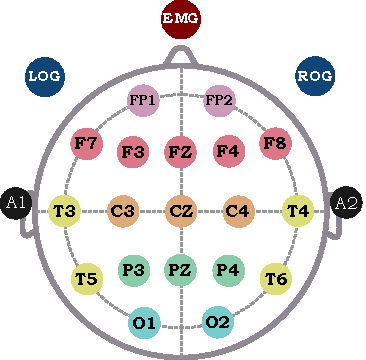
\includegraphics[scale=1.2]
{./img_diagramas/estampa_v1.pdf}
\caption{Representación minimalista de los electrodos considerados en el registro de PSG;
%: 19 para el EEG, dos para el EOG, un grupo de 3 para el EMG y dos electrodos de referencia.
para más detalles ver las secciones \ref{sec:eeg} y \ref{sec:emg_eog}.
Esta forma de ordenar las gráficas será usado en gráficos posteriores.}
\label{img:estampa}
\end{figure}

\begin{figure}
\centering
\begin{tabular}{c}
\begin{tabular}{cccc}
MJH & JAE & MGG & EMT \\
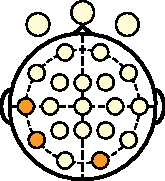
\includegraphics[width=0.17\textwidth]{./img_art_dfa/prop_MJH_30.pdf} &
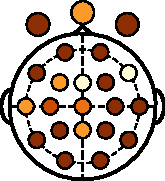
\includegraphics[width=0.17\textwidth]{./img_art_dfa/prop_JAE_30.pdf} &
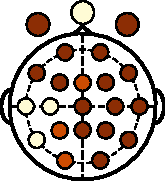
\includegraphics[width=0.17\textwidth]{./img_art_dfa/prop_MGG_30.pdf} &
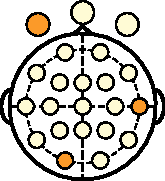
\includegraphics[width=0.17\textwidth]{./img_art_dfa/prop_EMT_30.pdf} \\
\end{tabular} \\
\midrule
\begin{tabular}{ccccc}
CLO & RLO & JGZ & AEFP & PCM \\
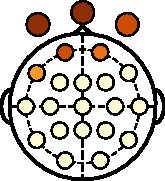
\includegraphics[width=0.17\textwidth]{./img_art_dfa/prop_CLO_30.pdf} &
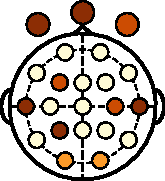
\includegraphics[width=0.17\textwidth]{./img_art_dfa/prop_RLO_30.pdf} &
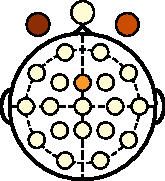
\includegraphics[width=0.17\textwidth]{./img_art_dfa/prop_JGZ_30.pdf} &
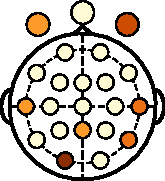
\includegraphics[width=0.17\textwidth]{./img_art_dfa/prop_AEFP_30.pdf} &
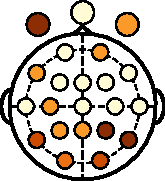
\includegraphics[width=0.17\textwidth]{./img_art_dfa/prop_PCM_30.pdf} \\
\end{tabular}
 \\

\includegraphics[scale=.7]{./img_art_dfa/escala.pdf} \\
\end{tabular}
\caption{Derivaciones para las cuales la proporción de épocas clasificadas como estacionarias fue significativamente diferente en MOR y NMOR.
%
En la parte superior se representa al grupo CTRL y en la parte inferior al grupo PDCL.
%
Para esta figura se usaron épocas de 30 segundos de duración.
%
La posición de los círculos representan a las derivaciones, en correspondencia con la figura \ref{img:estampa}.}
\label{cabeza_new}
\end{figure}

Con base a la hipótesis sobre estacionariedad local, discutida en la sección \ref{sec:est_local}, se procedió a repetir la clasificación de estacionariedad pero usando ventanas de diferentes tamaños.
%
Por fines de comparabilidad y por motivos técnicos, los tamaños de ventana se eligieron de la forma $30 \times 2^{n}$ segundos.
%
El tamaño de ventana más pequeño fue de $\nicefrac{30}{32}$ segundos para poder utilizar la prueba de PSR de forma confiable, mientras que el tamaño más grande fue de $120$ segundos tomando en cuenta que las ventanas más grandes serían demasiado heterogéneos para considerarse como unidades de estudio fiables.

En la figura \ref{cabeza_repoio} se muestra únicamente las proporciones estimadas de épocas estacionarias para MOR y NMOR ($\text{p}_{\text{MOR}}$ y $\text{p}_{\text{NMOR}}$) para un participante; los gráficos construidos para todos los participantes puede encontrarse en el apéndice \ref{apendiceA}.
%
Usando épocas de mayor duración, se encuentra que una proporción menor de estas son clasificadas como estacionarias; sin embargo, usando épocas de menor duración no se garantiza el efecto contrario.
%
Dicho fenómeno \textit{apoya} a la hipótesis de estacionariedad local en los registros de PSG en adultos mayores, aunque no representa evidencia suficiente para relacionarlo con el PDCL.

\begin{figure}
\centering
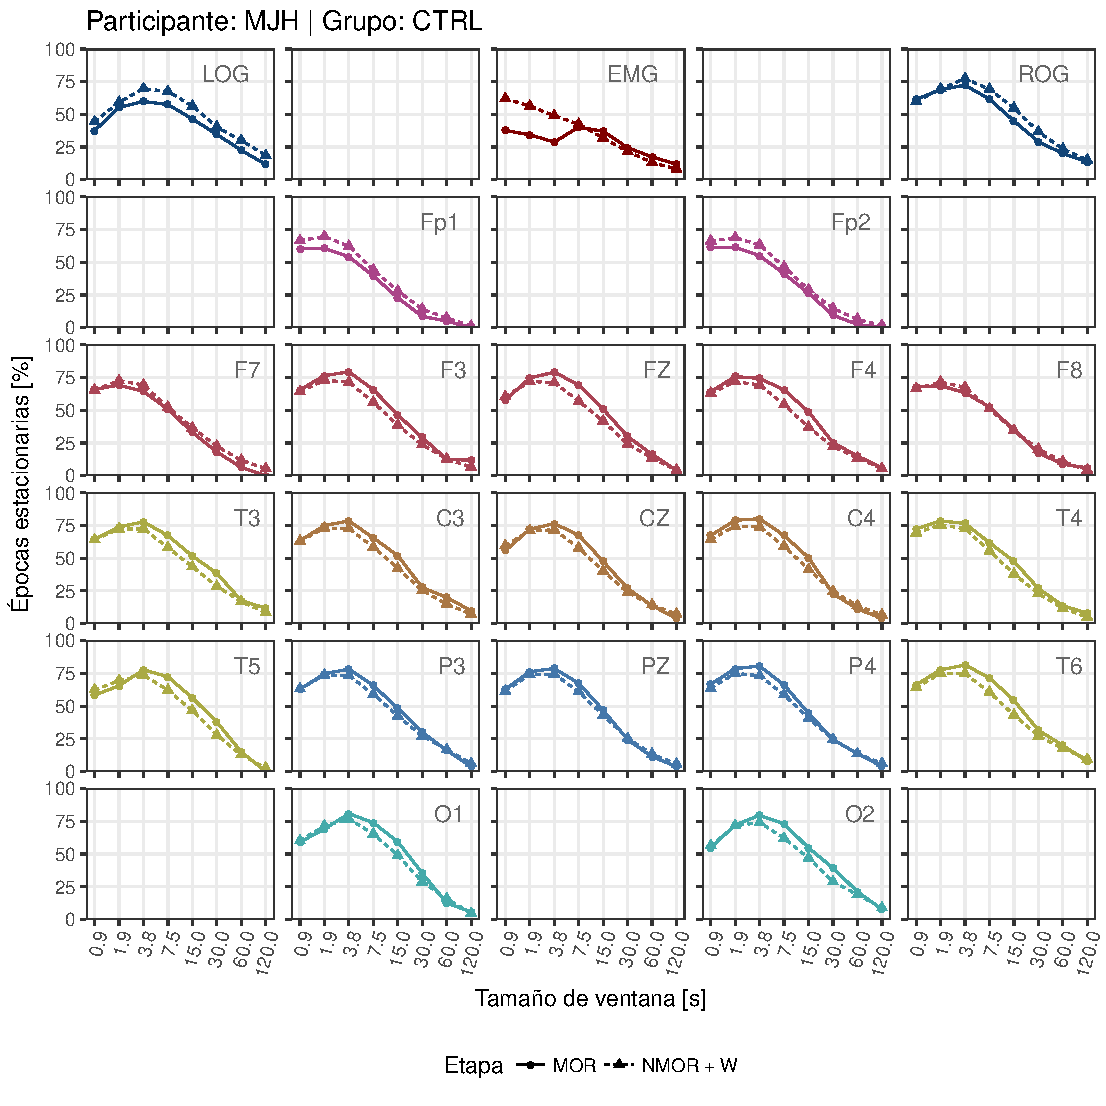
\includegraphics[width=\linewidth]{./scripts_graf_res/MJNNVIGILOS_cabeza_epocas_v2.pdf}
\caption{Cambio en la proporción de épocas estacionarias respecto al tamaño de ventana usado, durante MOR y NMOR. El análisis se repite en todas las derivaciones consideradas; la posición y color de cada gráfico se corresponden a aquellos de la figura \ref{img:estampa}. Sea abrevia W = vigilia, recordando que la cantidad tiempo de los registros clasificada como vigilia es negligible.}
\label{cabeza_repoio}
\end{figure}

En resumen, no se pudo identificar una conexión clara entre el PDCL y las características de las épocas como unidades autónomas.
%
Debido a ello se consideran otros niveles de organización sobre los registros: los registros como un conjunto de épocas distribuidas en el tiempo con \textit{cierta estructura}, y al individuo como unidad en la variabilidad de dichas estructuras.
%
En particular sobre el último, si se supone que las cantidades descritas en esta sección son características \textit{representativas} de cada participante, entonces tiene sentido intentar verificar similitudes con otros participantes o correlaciones con otras observaciones.

%%%%%%%%%%%%%%%%%%%%%%%%%%%%%%%%%%%%%%%%%%%%%%%%%%%%%%%%%%%%%%%%%%%%%%%%%%%%%%%%%%%%%%%%%%%%%%%%%%%
%%%%%%%%%%%%%%%%%%%%%%%%%%%%%%%%%%%%%%%%%%%%%%%%%%%%%%%%%%%%%%%%%%%%%%%%%%%%%%%%%%%%%%%%%%%%%%%%%%%

\section{Análisis a nivel de registro}
\label{sec:analisis_registro}

Como se mencionó en la sección \ref{sec:pdcl_sueno}, se ha reportado cambios en la estructura del sueño en adultos mayores con deterioro cognitivo, respecto a adultos mayores saludables.
%
El objetivo de esta subsección es intentar detectar estos \textit{cambios de estructura} usando los métodos descritos y bajo las condiciones descritas.

Con el fin de explorar cómo se relacionan las épocas estacionarias con la \textit{estructura del sueño}, se procedió a \textit{graficar} la estacionariedad.
%
Para efectuar lo anterior se consideró una cuadrícula, con una fila por cada derivación y una columna por cada época analizada (se registró el mismo número de épocas para cada derivación); sobre la cuadrícula el espacio correspondiente a cada época fue coloreado a según la clasificación de la época como estacionaria.
%
Se procedió similarmente para ilustrar la clasificación según etapa de sueño.
%
En la figura \ref{img:patrones} se ejemplifica este tipo de gráficos, además de otros detalles a mencionarse.

\begin{figure}
\centering
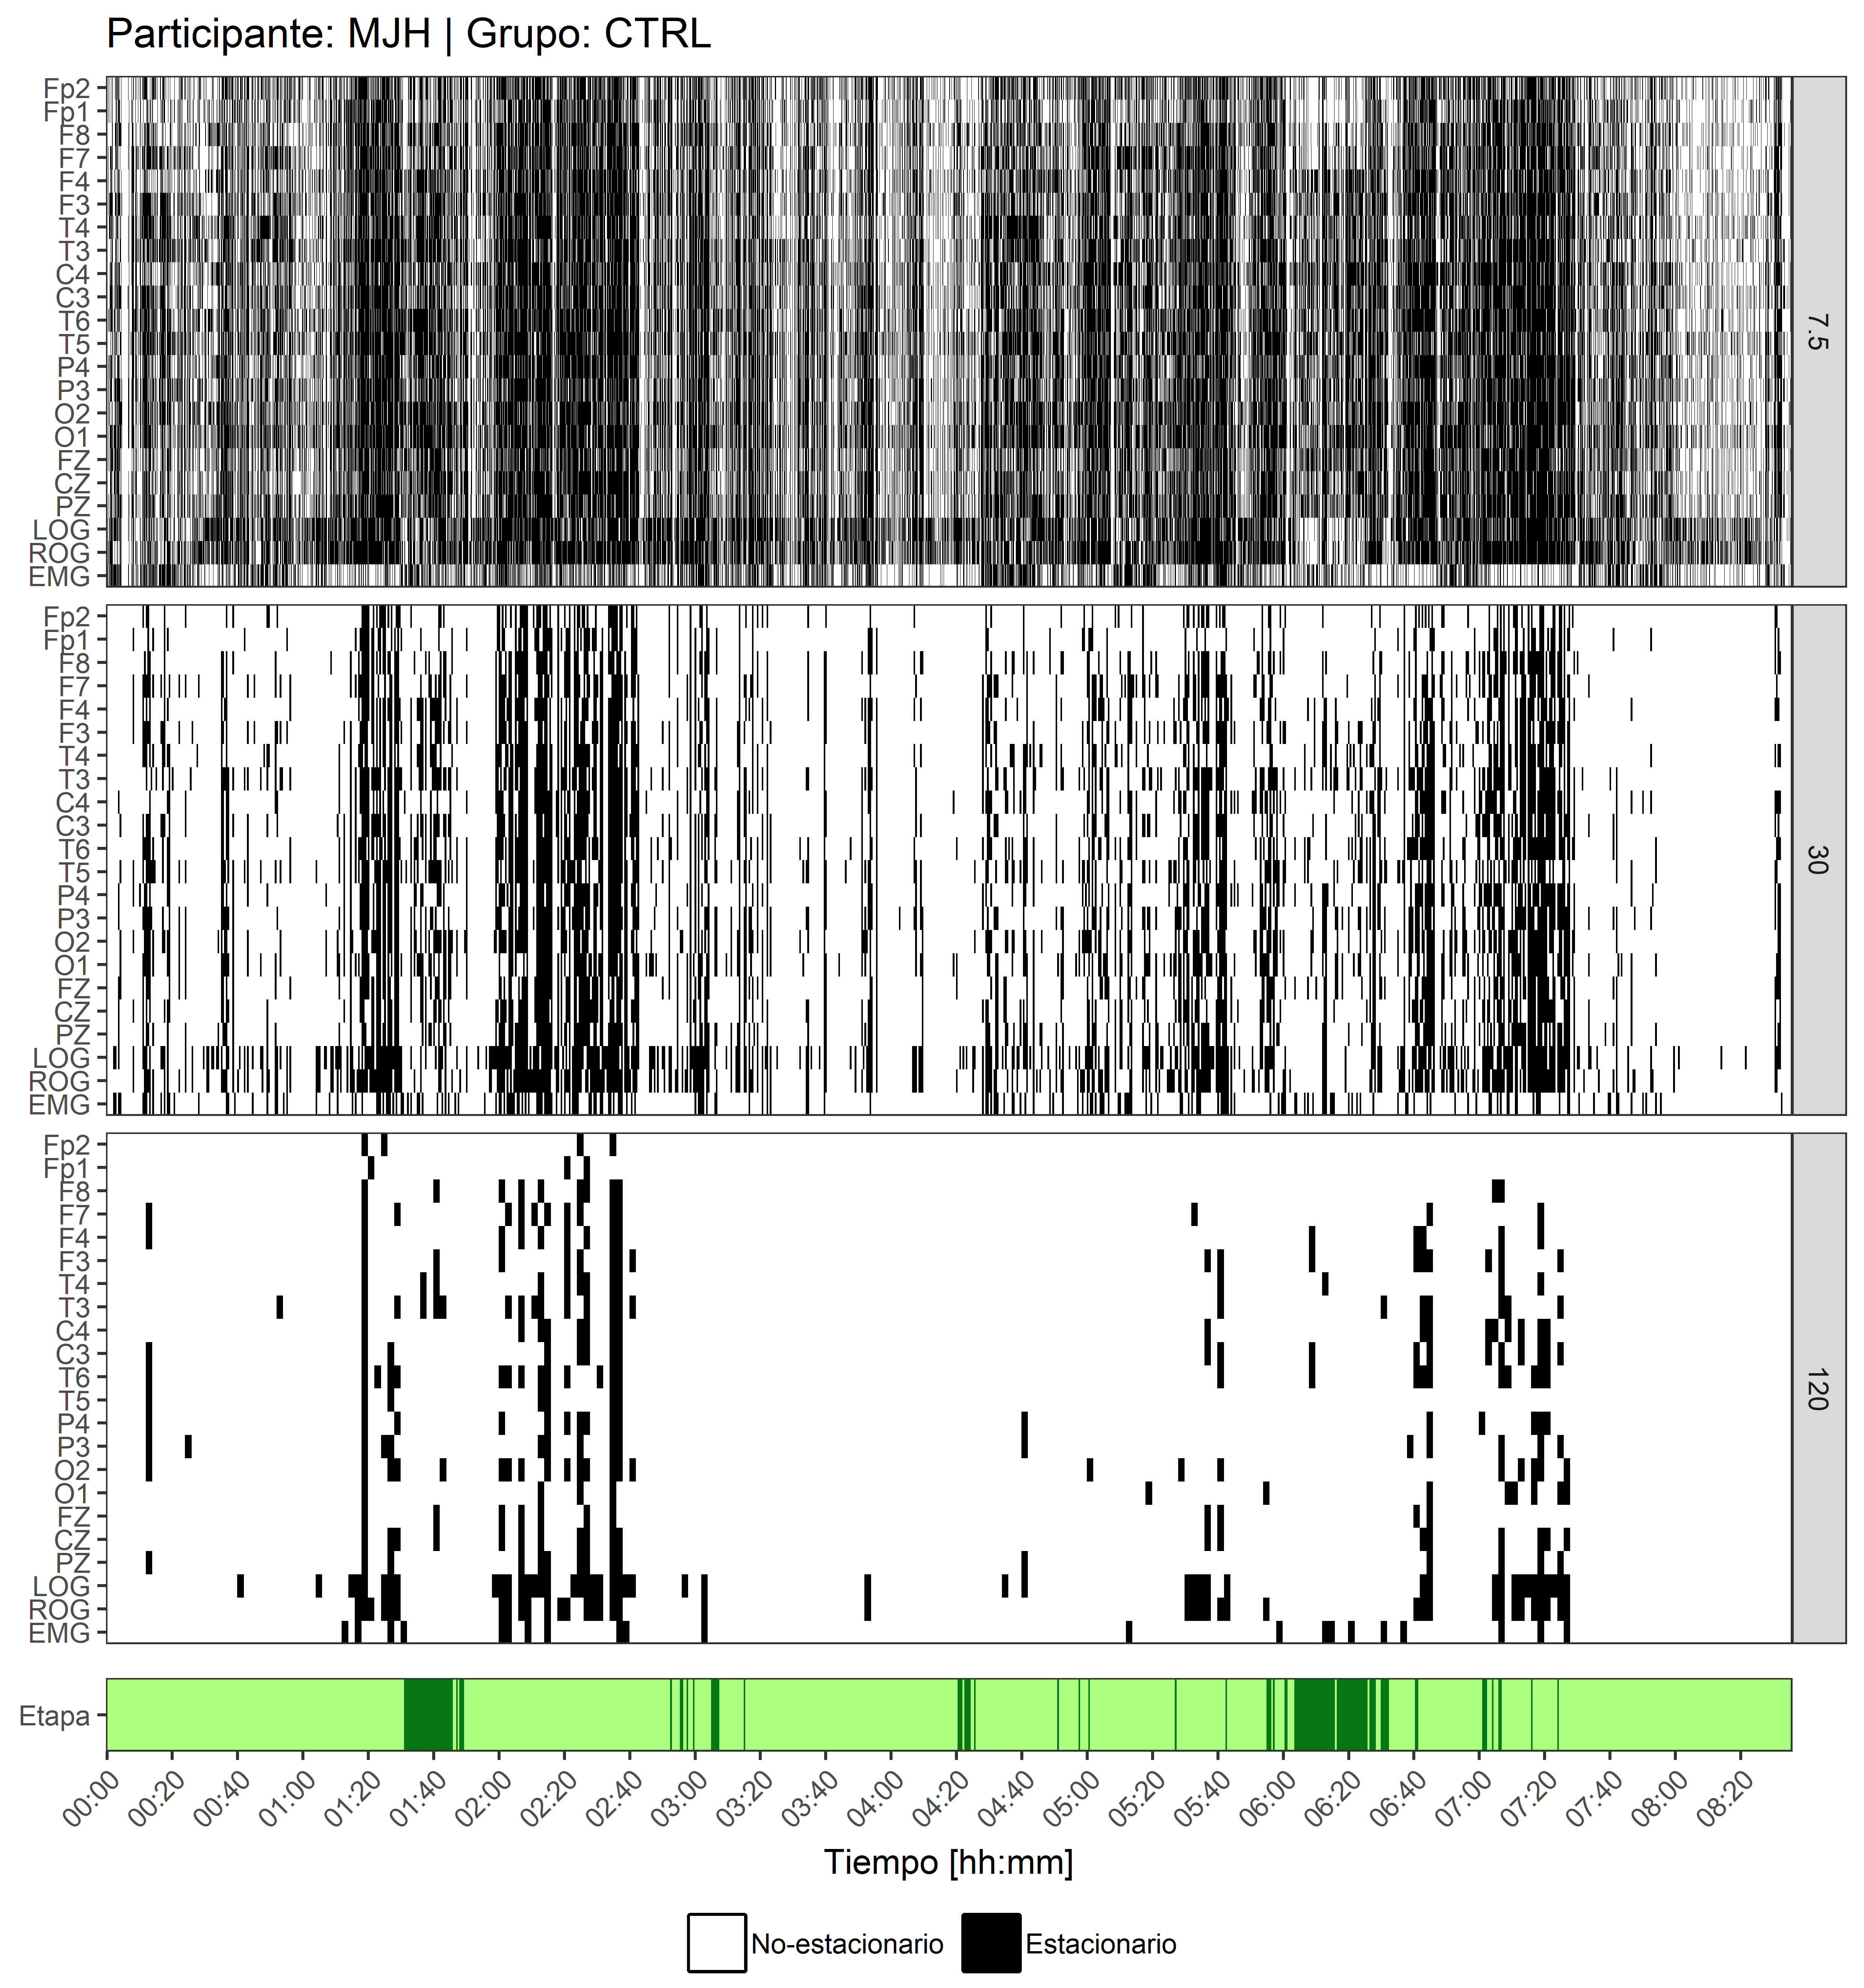
\includegraphics[width=\linewidth]
{./scripts_graf_res/MJNNVIGILOS_patrones_show.png}
\caption[Distribución en el tiempo de las ventanas clasificadas como estacionarias, considerando diferentes tamaños de ventana]{Distribución en el tiempo de las ventanas clasificadas como estacionarias, considerando diferentes tamaños de ventana. 
Cada ventana fue representada en una cuadrícula según su derivación (margen izquierdo) y momento (margen inferior) de procedencia; posteriormente fue \textit{coloreada} según su clasificación como estacionaria.
Dado que la clasificación de estacionariedad se repitió usando diversos tamaños de ventana, éstos se indican en el margen derecho.
En la parte inferior se representan las mismas épocas en su clasificación según etapa de sueño.
%Adicionalmente, en la parte superior se indican los \textit{patrones emergentes} de estacionariedad; para más detalles al respecto, ver el texto.
}
\label{img:patrones}
\end{figure}

Los gráficos obtenidos mediante este procedimiento mostraron algunas regularidades que merecen especial atención: \textit{bloques emergentes} de épocas que comparten clasificación como estacionarias (o como no--estacionarias).
%
Estos bloques identificados visualmente se extienden entre diversas derivaciones; puede verse un ejemplo de ello en la figura \ref{img:patrones}.
%
Debido a la forma en que se efectuó la clasificación de estacionariedad (usando la prueba de PSR) puede garantizarse que estos patrones emergentes no son producidos por la clasificación per se.
%
Se hipotetiza que estos \textit{patrones de estacionariedad}
corresponden a las diferentes etapas de sueño.
%
Posteriormente se discutirá con más detalle al respecto.

El procedimiento de graficación se repitió para las clasificaciones de estacionariedad obtenidas usando diferentes tamaños de ventana, con el fin de verificar si la presencia de los bloques podría atribuirse al tamaño de ventana usado.
%
Se encontró que los patrones aparecen con mayor o menor \textit{nitidez} en los gráficos obtenidos usando diferentes tamaños de ventana, tal como se ilustra en la figura \ref{img:patrones}.

%\begin{figure}
%\centering
%\includegraphics[width=.9\textwidth]
%{./img_art_dfa/zoom_noVCR_v2.png} \\
%\includegraphics[width=.9\textwidth]
%{./img_art_dfa/zoom_siVCR_v2.png}
%\caption[Ubicación de épocas estacionarias en el tiempo y patrones emergentes]
%{Ubicación de épocas estacionarias en el tiempo y patrones emergentes. \textbf{Arriba:} 
%Ubicación de épocas estacionarias en el tiempo.
%\textbf{Abajo:} Patrón de bloques relacionado con el sueño MOR}
%\label{patroncito}
%\end{figure}

%Usando la clasificación de épocas estacionarias, obtenida para diferentes tamaños de ventana, se 
%construyeron más gráficos sobre la ubicación de épocas estacionarias en el tiempo. Estos nuevos
%gráficos, como el de la figura \ref{comp_VCR}, refuerzan heurísticamente la hipótesis de que los 
%patrones son significativos fisiológicamente. 

%Entonces, se propone que los registros de PSG se comportan como procesos localmente estacionarios; 
%más aún, se propone que esta característica cambia cualitativamente en adultos mayores con PDC,
%para los cuales el \textit{nivel de homogeneidad} del PSG es muy similar durante MOR y NMOR.

%\begin{figure}
%\centering
%\includegraphics[width=\linewidth]
%{./img_art_dfa/VCNNS1_comp_est_.png}
%\caption{Distribución en el tiempo de ventanas estacionarias, usando diferentes tamaños
%de ventana.}
%\label{comp_VCR}
%\end{figure}

Dentro del contexto del PDCL en adultos mayores, estos patrones de estacionariedad no serán definidos formalmente ni estudiados detalladamente; se presentan como un hallazgo incidental y como verificación empírica de las capacidades de la técnica descrita para distinguir características que varían en el tiempo.
%
Esta decisión fue tomada considerando la naturaleza fuertemente cualitativa de dichos patrones.

%%%%%%%%%%%%%%%%%%%%%%%%%%%%%%%%%%%%%%%%%%%%%%%%%%%%%%%%%%%%%%%%%%%%%%%%%%%%%%%%%%%%%%%%%%%%%%%%%%%

\section{Análisis a nivel de grupo}

Para fines de esta subsección, se ha supuesto que las proporciones de épocas estacionarias durante MOR y NMOR ($\text{p}_{\text{MOR}}$ y $\text{p}_{\text{NMOR}}$) son características intrínsecas de cada individuo. 
%
En otras palabras, si se repite el registro de PSG para el mismo individuo y bajo condiciones similares, y se realiza el mismo procedimiento de segmentación y clasificación de épocas, entonces se espera que las cantidades $\text{p}_{\text{MOR}}$ y $\text{p}_{\text{NMOR}}$ serán las mismas.
%
Este supuesto se basa en que las fases de sueño son \textit{casi indistinguibles} entre diferentes individuos con características similares, y más aún entre diferentes jornadas de sueño para el mismo individuo.
%; para un estudio más detallado de estas últimas afirmaciones, consultar el libro \textit{``Psicofisiología del sueño"} \cite{Corsi1983}.

Con base a los resultados de la subsección anterior, se puede afirmar intuitivamente que la metodología descrita \textit{percibe} parte de algunas fases (o subfases) de sueño, las cuales son comunes entre individuos.
%
Sin embargo, aun si tales observaciones fueran verificadas rigurosamente, el supuesto de que $\text{p}_{\text{MOR}}$ y $\text{p}_{\text{NMOR}}$ son características individuales debería ser verificado por separado.
%
Debido a las limitaciones del presente trabajo --especialmente el tamaño muestral reducido y la limitación de un registro por participante-- el supuesto será usado como tal, y no se verificará debido a la falta de datos.
%
En consecuencia, los resultados en la presente subsección se presentan como \textit{indicios}, con la idea de explorarlos en trabajos futuros.

Entonces bien, las cantidades $\text{p}_{\text{MOR}}$ y $\text{p}_{\text{NMOR}}$, calculadas por separado para todos los participante y todas las derivaciones consideradas, fueron tratados como características que se distribuyen de forma aproximadamente normal sobre las poblaciones que representan los grupos CTRL y PDCL.
%
Se efectuó un ANOVA de dos vías para observar los cambios sobre $\text{p}_{\text{MOR}}$ y $\text{p}_{\text{NMOR}}$ debidos al grupo y la etapa de sueño, cuyos resultados se muestran en el cuadro \ref{tabla:anova_prop}.
%
Se encontró que no hay interacciones significativas entre los factores de etapa y grupo para ninguna derivación; así mismo se encontró que hay diferencias significativas para las derivaciones Fp2, F7, LOG y ROG que pueden ser explicadas por el \textit{efecto} de la etapa se sueño, y de forma similar para las derivaciones LOG y ROG con el efecto de grupo.

Las diferencias para LOG y ROG debido, debidas al efecto de `etapa de sueño', puede explicarse perfectamente por la presencia característica de movimientos oculares rápidos en el sueño MOR; en cierto sentido, este resultado era de esperarse.
%
Las diferencias en Fp2 y F7 requieren una explicación más cautelosa, ya que el efecto es significativo en la región frontal, la cual típicamente es asociada con la toma de decisiones; sin embargo, la \textit{significancia} es débil y no es consistente sobre la región frontal.
%
Para explorar más a fondo los resultados de la ANOVA, en la figura \ref{comparacion_verde} se han graficado (como diagramas de caja) los valores $\text{p}_{\text{MOR}}$ y $\text{p}_{\text{NMOR}}$ muestrales; se observa que intuitivamente las cantidades $\text{p}_{\text{MOR}}$ y $\text{p}_{\text{NMOR}}$ entre grupos y entre etapas, pero no resultan significativas debido a la gran variablidad dentro de las categrorías.
%
En principio es posible justificar dicha falla por una muestra muy pequeña.

Con respecto a las diferencias entre grupos para las derivaciones LOG y ROG, puede decirse que recientemente se ha sugerido que es posible detectar diferencias entre sujetos con y sin DCL usando registros de --entre otras derivaciones-- movimientos oculares [articulo??].

\begin{SidewaysTable}
\centering
\caption{ANOVA para los efectos Grupo y Etapa de sueño sobre las cantidades $\text{p}_{\text{MOR}}$ y $\text{p}_{\text{NMOR}}$.}
\label{tabla:anova_prop}
\begin{tabular}{lllllllllllllrllrllrl}
\toprule
 & \multicolumn{5}{l}{CTRL} &  & \multicolumn{5}{l}{PDCL} &  & \multicolumn{8}{l}{ANOVA} \\
\cmidrule{2-6} \cmidrule{8-12} \cmidrule{14-18}
 & \multicolumn{2}{l}{NMOR} &  & \multicolumn{2}{l}{MOR} &  & \multicolumn{2}{l}{NMOR} &  & \multicolumn{2}{l}{MOR} &  & \multicolumn{2}{l}{Grupo} &  & \multicolumn{2}{l}{Etapa} &  & \multicolumn{2}{l}{G$\times$E} \\
\cmidrule{2-3} \cmidrule{5-6} \cmidrule{8-9} \cmidrule{11-12} \cmidrule{14-15} \cmidrule{17-18} \cmidrule{20-21} 
 & M & DE & & M & DE & & M & DE & & M & DE & & F & p & & F & p & & F & p \\
\midrule
Fp2 & .172 & .040 &  & .063 & .058 &  & .106 & .084 &  & .037 & .070 &  & 2.08 & .171 &  & 7.51 & .016 &  & .40 & .537 \\
Fp1 & .175 & .090 &  & .091 & .115 &  & .108 & .105 &  & .045 & .077 &  & 1.53 & .237 &  & 2.48 & .138 &  & .05 & .829 \\
F8 & .193 & .076 &  & .147 & .133 &  & .125 & .078 &  & .089 & .140 &  & 1.43 & .252 &  & .60 & .453 &  & .01 & .918 \\
F7 & .190 & .050 &  & .077 & .076 &  & .126 & .096 &  & .055 & .106 &  & 1.09 & .314 &  & 4.81 & .046 &  & .25 & .621 \\
F4 & .200 & .055 &  & .162 & .145 &  & .144 & .125 &  & .152 & .151 &  & .30 & .595 &  & .04 & .836 &  & .14 & .716 \\
F3 & .199 & .040 &  & .144 & .099 &  & .151 & .138 &  & .171 & .230 &  & .02 & .890 &  & .03 & .858 &  & .27 & .610 \\
T4 & .224 & .076 &  & .212 & .171 &  & .162 & .078 &  & .262 & .190 &  & .01 & .926 &  & .57 & .461 &  & .71 & .414 \\
T3 & .272 & .066 &  & .281 & .148 &  & .187 & .095 &  & .245 & .207 &  & .79 & .390 &  & .28 & .603 &  & .13 & .726 \\
C4 & .294 & .079 &  & .232 & .159 &  & .169 & .124 &  & .256 & .188 &  & .53 & .481 &  & .09 & .772 &  & 1.15 & .301 \\
C3 & .255 & .054 &  & .248 & .115 &  & .188 & .122 &  & .250 & .180 &  & .28 & .604 &  & .27 & .614 &  & .31 & .585 \\
T6 & .315 & .105 &  & .241 & .151 &  & .170 & .093 &  & .250 & .210 &  & .94 & .349 &  & .03 & .871 &  & 1.20 & .292 \\
T5 & .294 & .167 &  & .337 & .231 &  & .222 & .149 &  & .320 & .178 &  & .27 & .612 &  & .74 & .403 &  & .10 & .755 \\
P4 & .258 & .060 &  & .201 & .134 &  & .158 & .100 &  & .227 & .194 &  & .33 & .576 &  & .04 & .843 &  & .95 & .345 \\
P3 & .256 & .097 &  & .227 & .138 &  & .187 & .101 &  & .286 & .190 &  & .01 & .939 &  & .42 & .526 &  & .93 & .350 \\
O2 & .272 & .078 &  & .243 & .181 &  & .183 & .112 &  & .255 & .210 &  & .26 & .615 &  & .13 & .721 &  & .47 & .506 \\
O1 & .278 & .095 &  & .291 & .209 &  & .175 & .117 &  & .253 & .206 &  & .81 & .383 &  & .40 & .539 &  & .17 & .685 \\
FZ & .234 & .031 &  & .242 & .109 &  & .168 & .139 &  & .215 & .178 &  & .55 & .469 &  & .24 & .634 &  & .10 & .758 \\
CZ & .225 & .062 &  & .187 & .111 &  & .164 & .120 &  & .178 & .127 &  & .46 & .510 &  & .03 & .865 &  & .24 & .633 \\
PZ & .229 & .049 &  & .176 & .100 &  & .160 & .119 &  & .230 & .177 &  & .02 & .904 &  & .07 & .797 &  & 1.06 & .321 \\
LOG & .505 & .103 &  & .229 & .132 &  & .343 & .089 &  & .094 & .096 &  & 9.10 & .009 &  & 28.19 & .000 &  & .08 & .786 \\
ROG & .542 & .149 &  & .305 & .173 &  & .342 & .171 &  & .143 & .133 &  & 5.89 & .029 &  & 8.53 & .011 &  & .07 & .800 \\
EMG & .151 & .082 &  & .162 & .094 &  & .068 & .074 &  & .139 & .166 &  & .99 & .337 &  & .68 & .423 &  & .31 & .588 \\
\bottomrule 
\multicolumn{20}{l}{M=media muestral; SD=Desviación estándar; G$\times$E=interacción Grupo y Etapa}
\end{tabular}
\end{SidewaysTable}

\begin{figure}
\centering
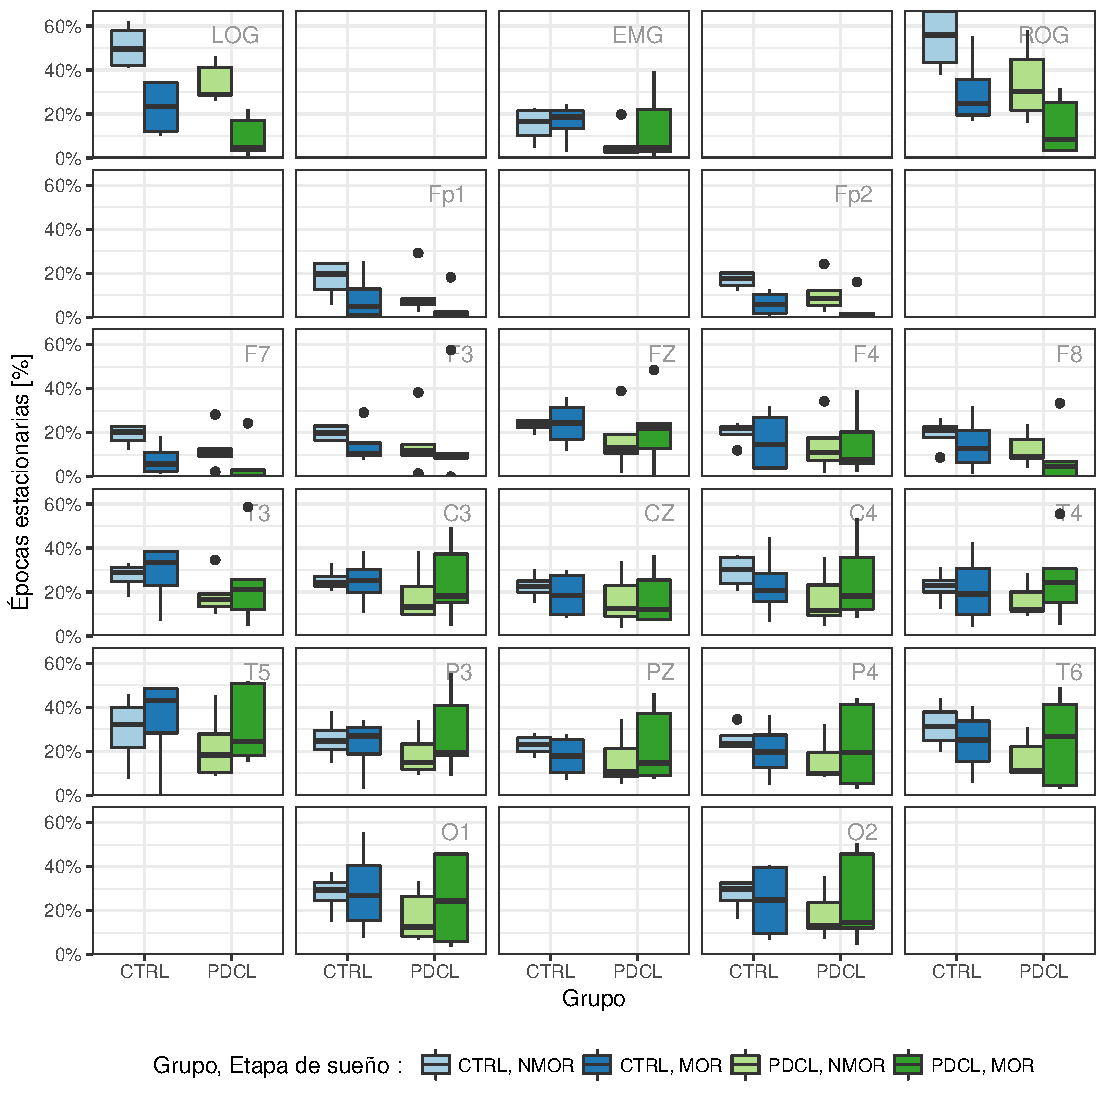
\includegraphics[width=\linewidth]
{./scripts_graf_res/comparacion_cabeza.pdf}
\caption{Proporciones de épocas estacionarias, durante sueño MOR y NMOR y para todas las derivaciones.
%
Los puntos representan valores \textit{atípicos}, según su definición para diagramas de caja (ver sección ??).
%; es decir, aquellos valores fuera del intervalo $[Q_1-1.5 R, Q_3 + 1.5 R]$, con $Q_1$ y $Q_3$ el primero y tercer cuartiles muestrales y $R=Q_3-Q_1$.
%
La posición de cada gráfico se corresponden con aquellos de la figura \ref{img:estampa}.}
\label{comparacion_verde}
\end{figure}

%\begin{figure}
%\centering
%\includegraphics[width=\linewidth]
%{./img_art_dfa/Comparacion_gpos_CTL_PDC_v3.pdf}
%\caption{Proporciones de épocas estacionarias, durante sueño MOR y NMOR.}
%\label{comparacion_verde}
%\end{figure}
%
%\begin{figure}
%\centering
%\includegraphics[width=\linewidth]
%{./img_art_dfa/Comparacion_gpos_MOR_NMOR_v3.pdf}
%\caption{Proporciones de épocas estacionarias, grupos CTL y PDC.}
%\label{comparacion_graf}
%\end{figure}

%%%%%%%%%%%%%%%%%%%%%%%%%%%%%%%%%%%%%%%%%%%%%%%%%%%%%%%%%%%%%%%%%%%%%%%%%%%%%%%%%%%%%%%%%%%%%%%%%%%
%%%%%%%%%%%%%%%%%%%%%%%%%%%%%%%%%%%%%%%%%%%%%%%%%%%%%%%%%%%%%%%%%%%%%%%%%%%%%%%%%%%%%%%%%%%%%%%%%%%
%%%%%%%%%%%%%%%%%%%%%%%%%%%%%%%%%%%%%%%%%%%%%%%%%%%%%%%%%%%%%%%%%%%%%%%%%%%%%%%%%%%%%%%%%%%%%%%%%%%
%%%%%%%%%%%%%%%%%%%%%%%%%%%%%%%%%%%%%%%%%%%%%%%%%%%%%%%%%%%%%%%%%%%%%%%%%%%%%%%%%%%%%%%%%%%%%%%%%%%